%--------------------------- Hoda Abbasi ----------------------------
%----------------------- 10 November 2015 ------------------------

\documentclass[12pt]{book}

\usepackage{a4}
\usepackage[graph]{xy}
\usepackage{graphicx}
\input Latex_macros/Definitionen.tex
\setcounter{tocdepth}{4}
\setcounter{secnumdepth}{4}
\usepackage{enumerate}
\usepackage[active]{srcltx}
\newcommand{\Schrift}{report}
%\newcommand{\Schrift}{book}
%--------------------------------------------------------------------------------------------------------------------------------------

\begin{document}
\title{\bf \Huge Report}

\author{ \bf Hoda Abbasi\\
 PhD Candidate\\
 Computer Science Department\\
Swansea University\\
}
\maketitle
%--------------------------------------------------------------------------------------------------------------------------------------
\tableofcontents
%\chapter{Internal organisation}
%\label{cha:Internalorganisation}

%\section{Overview on questions and conjectures}
%\label{sec:Overview on questions and conjectures}

%\begin{description}
%\item 
%\end{description}
%--------------------------------------------------------------------------------------------------------------------------------------
%\part{Preparations}
%\label{par:Preparations}
%***************************************************************************************************************************************************************
%***************************************************************************************************************************************************************

\chapter{Set Theory}
\label{cha:settheory}

%--------------------------------------------------------------------------------------------------------------------------------------
\section{Ontological Preparations}
%\label{sec:Ontological preparations}

A \textbf{thing} is in general fuzzy, perhaps escapes precise definition at all. An \textbf{object} is a clearly defined, clearly outlined thing. A \textbf{theory} is about a realm of objects.
\textbf{Mathematical objects} are for example various types of numbers and spaces. In set theory, every mathematical object is given to us as a \textbf{set}.
%--------------------------------------------------------------------------------------------------------------------------------------

\section{Naive Set Theory}
\label{sec:Naivesettheory}

Pure set theory has exactly one type of object, called ``set'', and thus everything is a set here  \cite{h1}. We find it useful to use an extension, where there are ``sets'' and urelements, that is, objects are either urelements (``atomic'') or sets.
\begin{examp}\label{exp:urelemente}
If we want to assume ``numbers'', like $\NNZ \subset \NN \subset \ZZ \subset \QQ \subset \RR \subset \CC$, then we can consider them as urelements, that is, they are already given (from the outside), and they have no internal structure, that is, none of these numbers have elements; compare Section \ref{def:natnumberssimple} for the alternative approach of of defining $\NNZ = \omega$ via sets.
\end{examp}
Intuitively, a set is a ``collection'' of objects, that is, a ``collection'' of sets and urelements. ``Collection'' here means a set $x$ (not an urelement), such that for every object $y$ it can be said, whether $y$ is an element of $x$, that is, ``\bmm{y \in x}'', or $y$ is not an element of $x$, that is, ``\bmm{y \notin x}''. Thus there is no order on the elements of a set, and an object can not be multiple times in a set (it is just ``in or out''). 
Two objects $x, y$ can be compared for equality, that is, we either have \bmm{x = y} or \bmm{x \ne y}. Since a set is given by its elements, we have $x = y$ for sets $x, y$ iff for all objects $z$ holds $z \in x \Lra z \in y$, while we have $x \ne y$ iff there is an object $z$ with $z \in x$ but $z \notin y$, or $z \in y$ but $z \notin x$.
For an urelement $x$ and every object $y$ holds $y \notin x$. Urelements can be compared by equality, where this relation is atomic (given).

\begin{defi}\label{def:sse}
  For sets $x, y$ holds \bmm{x \sse y} if for all objects $z \in x$ holds $z \in y$, while \bmm{x \subset y} holds if $x \sse y$ and $x \ne y$.
\end{defi}
Remarks:
% enumerate is used to create a numbered list
\begin{enumerate}
\item So $x = y$ iff $x \sse y$ and $y \sse x$.
\item And $x \subset y$ iff for all elements $z \in x$ holds $z \in y$, while there is a $z' \in y$ with $z' \notin x$.
\item \cite{h2} uses ``$\subset$'' instead of ``$\sse$''.
\end{enumerate}

%--------------------------------------------------------------------------------------------------------------------------------------
\subsection{Set Formation}
\label{sec:setformation}

Given objects $x, y$ we can form the \textbf{singleton} \bmm{\set{x}} and the \textbf{2-set} \bmm{\set{x,y}}, that is, sets, where for every object $z$ holds:
\begin{enumerate}
\item $z \in \set{x} \Lra z = x$;
\item $z \in \set{x,y} \Lra z = x \vee z = y$.
\end{enumerate}

More fundamentally, there is the \textbf{empty set} \bmm{\es}, characterised by the property, that for all objects $x$ holds $x \notin \es$.

Given sets $x, y$, we can form three further sets:
\begin{itemize}
\item the \textbf{union} \bmm{x \cup y}, characterised by $\fa\, z : z \in x \cup y \Lra z \in x \vee z \in y$;
\item the \textbf{intersection} \bmm{x \cap y}, characterised by $\fa\, z : z \in x \cap y \Lra z \in x \wedge z \in y$;
\item the \textbf{(set-)difference} \bmm{x \sm y}, characterised by $\fa\, z : z \in x \sm y \Lra z \in x \wedge z \notin y$.
\end{itemize}
Remarks:
\begin{enumerate}
 \item Intersection and union operation are {\it commutative} and {\it associative}.
 \item For sets $x, y, z$ we have the following properties \cite{h1}.
  \begin{enumerate}
  \item $x - \emptyset = x\ ;\ x - x = \emptyset $. 
  \item $x \cup x = x\ ;\ x \cap x = x $.
  \item $x \subseteq x \cup y\ ;\ x \cap y \subseteq x$.
  \item $x \cup (y \cap z) = (x \cup y) \cap (x \cup z)$.
  \item $x \cap (y \cup z) = (x \cap y) \cup (x \cap z)$.
  \item $(x \subseteq y) \leftrightarrow (x \cap y=x) \leftrightarrow (x \cup y = y)$.
  \item $x - y = x - (x \cap y)$.
  \end{enumerate}
  \item Two sets are said to be \bmm{disjoint} if they have no member in common; in symbols \cite{h1},
    $$ x \cap y = \emptyset .$$
  \item If $x, y $ are subset of $z$ , we have the following properties:
    \begin{enumerate}
	\item $z - ( z - x ) = x$;
	\item $(x \subseteq y) \leftrightarrow [(z - y) \subseteq (z - x)]}$;
	\item $x \cup (z - x) = z$;
	\item $z - (x \cup y) = (z - x) \cap (z - y)$;
	\item $z - (x \cap y) = (z - x) \cup (z - y)$.
	\end{enumerate}
  \item From the {\it axiom of extensionality}, it is proved that there is only one empty set \cite{h1}.
\end{enumerate}
%--------------------------------------------------------------------------------------------------------------------------------------
\subsection{(Ordered) Pairs}
\label{sec:ordpairs}

\begin{defi}\label{def:pairs}
  For objects $x, y$ we define the \textbf{pair} \bmm{(x,y)} via
  \begin{displaymath}
    (x,y) := \set{\set{x},\set{x,y}}.
  \end{displaymath}
  A set $x$ is called \textbf{a pair}, if there are objects $y,z$ with $x = (y,z)$.
\end{defi}
Remarks:
\begin{enumerate}
\item If $x=y$, then $(x,y) = \set{\set{x}}$.
\item For example, $\es$ is not a pair.
\end{enumerate}
\begin{lem}\label{lem:pairs}
  For objects $x, y, x', y'$ holds $(x,y) = (x',y') \Lra x = x' \wedge y = y'$.
\end{lem}

\begin{defi}\label{def:projpairs}
  For a pair $x$ we define the object \bmm{\proj_1(x)}, \bmm{\proj_2(x)} as those unique objects with $x = (\proj_1(x), \proj_2(x))$ (``projections'').
\end{defi}

%--------------------------------------------------------------------------------------------------------------------------------------

\subsection{Product of Sets}
\label{sec:productsets}

\begin{defi}\label{def:productsets}
  For sets $X, Y$ the set of all pairs $x, y$ with $x \in X$ and $y \in Y$ exists and is denoted by
  \begin{displaymath}
    \bmm{X \times Y} := \set{(x,y): x \in X \wedge y \in Y}.
  \end{displaymath}
\end{defi}
Remarks:
\begin{enumerate}
 \item For sets $A, B, C, D$ we have the following properties.
  \begin{enumerate}
  \item\label{thm:propprod5} $A \times \emptyset = \emptyset \times A = \emptyset$.
  \item\label{thm:propprod1} $A \times (B \cap C) = (A\times B) \cap (A \times C)$.
  \item\label{thm:propprod2} $A \times (B \cup C) = (A \times B) \cup (A \times C)$.
  \item\label{thm:propprod3} $(A \times B) \cap (C \times D) = (A \cap C) \times (B \cap D)$.
  \item\label{thm:propprod4} $(A \times B) \cup (C \times D) \subseteq (A \cup C) \times (B \cup D)$.
  \end{enumerate}
\end{enumerate}
%--------------------------------------------------------------------------------------------------------------------------------------

\subsection{Infinitary Set Constructions}
\label{sec:Infinitary set constructions}

\begin{itemize}
\item A \textbf{set system} is a set $X$, such that for all $y \in X$ holds that also $y$ is a set (all elements are sets). For a set system $X$ the \textbf{union} \bmm{\bc X} is characterised by $x \in \bc X \Lra \ex\, y \in X : x \in y$.
\item For a set $x$ there is the \textbf{power set} \bmm{\pot(x)}, characterised by $y \in \pot(x) \Lra y \sse x$ for sets $y$ (the power set is the set of all subsets). So a powerset is a set system.
\item If $x$ is a set, and $\Phi(y)$ a property of a set variable $y$ (a logical formula), then $\set{y \mb y \in x \wedge \Phi(y)}$ is a set, characterised by the property, that the elements of it are precisely those $y$ with $y \in x$ and $\Phi(y)$. In this way we can form specific subsets (via \textbf{comprehension}).
\item If $X$ is a set, and $F(x)$ a specification of a unique object for all $x \in X$, then we have the set $\set{F(x) \mb x \in X}$, which is the set of all objects $y$, such that there is some $x \in X$ with $y = F(x)$. This is a form of image (via \textbf{replacement}).
\end{itemize}

\begin{examp}\label{exp:infset}
 For set $A= \{1,2\}$ the power set is : $\pot(A)=\{ \emptyset,\{1\},\{2\},\{1,2\}\}$.
\end{examp}
%--------------------------------------------------------------------------------------------------------------------------------------
\subsection{Relations and Maps}
\label{sec:maps}

\begin{defi}\label{def:reli}
  A \textbf{relation} is a set of pairs. The \textbf{first projection} of a relation $R$ is $\bmm{\proj_1(R)} := \set{\proj_1(p) : p \in R}$, the \textbf{second projection} is $\bmm{\proj_2(R)} := \set{\proj_2(p) : p \in R}$. For a relation $R$ and a set $X$ one defines $\bmm{R(X)}:= \set{y \in \proj_2(R) \mb \ex\, x \in X : (x,y) \in R}$ (the ``image'' of $X$ under $R$).
\end{defi}
Remarks:
\begin{enumerate}
\item Instead of ``second projection'' one might also use ``range''. However for the first projection to use ``domain'' is misleading, since a relation does not need to have every element of the domain in its first projection (different from a map).

  The notations $\proj_i(R)$ for $i \in \tb{1,2}$ can be understood as a special case of the notation ``$R(X)$'', but where $R$ is not a set.
\item $\es$ is a relation, and for all sets $X$ holds $\es(X) = \es$.
\end{enumerate}

\begin{defi}\label{def:map}
  A \textbf{map} is a relation $f$ such that for all $x \in \proj_1(f)$ there is exactly one $y \in \proj_2(F)$ with $(x,y) \in f$, where then $y =: \bmm{f(x)}$ is used. Furthermore $\bmm{\dom(f)} := \proj_1(f)$ (``domain'') and $\bmm{\rg(f)} := \proj_2(f)$ (``range'').
\end{defi}
Remarks:
\begin{enumerate}
\item Normally there is no confusion between $f(X) = \set{f(x) : x \in X \cap \dom(f)}$ for a set $X$ according to Definition \ref{def:reli}, and $f(x) = y$ for a \emph{single} argument $x \in \dom(f)$.
\end{enumerate}
%--------------------------------------------------------------------------------------------------------------------------------------

\subsection{Special Maps}
\label{sec:Specialmaps}

\begin{defi}\label{def:inj}
  A map $f$ is called an \textbf{injection} (``is injective'') if for all $x, x' \in \dom(f)$ holds $f(x) = f(x') \Ra x = x'$.
\end{defi}

\begin{defi}\label{def:surj}
  For a map $f$ holds the statement \bmm{f:X \ra Y} if $X, Y$ are sets with $X = \dom(f)$ and $\rg(f) \sse Y$. Such a statement attaches to \textbf{codomian} (or ``target set'') $Y$ to the map $f$. Given such a codomain $Y$, $f$ is called \textbf{surjective} if $\rg(F) = Y$.
\end{defi}

\begin{defi}\label{def:bij}
  A map $f$ with codomain $Y$ is called \textbf{bijective} (``is a bijection'') if $f$ is injective and surjective.
\end{defi}

Remarks:
\begin{enumerate}
\item If sets $A , B$ are injective and infinite, then we have $\abs{A} \leq \abs{B}$
\end{enumerate}
%?????????????????????
\begin{examp}\label{exp:Specialmaps}
  The map $F(x) = 3 x + 7$ is injective but the map $G(x) = x^4 - x$ is not. Figure 1.1 showes another examples.
\end{examp}

\begin{figure}
   % \begin{center}
	\centering
       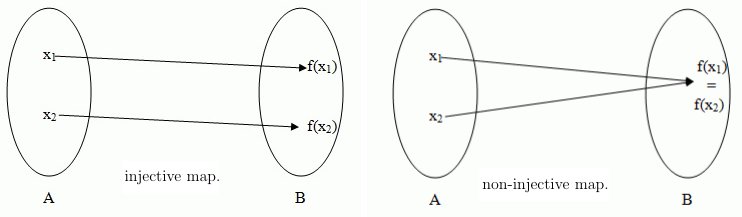
\includegraphics[scale =0.8]{p11.png}
       \caption{Examples of injective and non-injective map.}
    \end{center}
	
\end{figure}
\begin{examp}\label{exp:Specialmaps}
  The map $F(x) = 2 x $ from natural numbers to the set of non-negative even numbers is surjective but from the set of natural numbers to natural numbers is non-surjective.
\end{examp}
\begin{examp}\label{exp:Specialmaps}
  The map $F(x) = x^2$ from the set of positive numbers to positive real numbers is injective and surjective. Therefore, it is bijective.
\end{examp}



%\begin{figure}
    %\begin{center}
	%\centering
      % 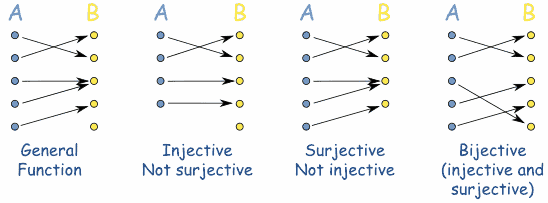
\includegraphics{p3.png}
      % \caption{Example of different typs of map.}
    %\end{center}
%\end{figure}
%--------------------------------------------------------------------------------------------------------------------------------------
\subsection{Decompositions and Equivalence Relations}
\label{sec:Decompositions}

\begin{defi}\label{def:Decompositions}
  A \textbf{partition} of a set $X$ is some $P \sse \pot(X) \sm \set{\es}$ wich is disjoint, i.e., $\fa\, A, B \in P : A \ne B \Ra A \cap B = \es$, and where $\bc P = X$.
\end{defi}
\begin{examp}\label{exp:Decompositions}
  The set $X = \{ 1, 2, 3 \} $ has these five partitions:
  $$ \{ \{1\}, \{2\}, \{3\}\}$$
  $$ \{ \{1,2\}, \{3\}\}$$
  $$ \{ \{1, 3\}, \{2\}\}$$
  $$ \{ \{1\}, \{2, 3\}\}$$
  $$ \{ \{ 1, 2, 3 \}\}$$
  The following are not partitions of X.
  $$ \{ \{\}, \{2, 3\}\}$$
  $$ \{ \{1, 2\}, \{2, 3\}\}$$
  $$ \{ \{1\}, \{2\}\}$$
\end{examp}
%--------------------------------------------------------------------------------------------------------------------------------------

\subsection{Finite Sets}
\label{sec:Finite sets}

\begin{defi}\label{def:finite}
  A set $X$ is called \textbf{infinite} if there is a bijection $f: X \ra X'$ for some $X' \subset X$, otherwise $X$ is called \textbf{finite}.
\end{defi}

\begin{defi}\label{def:finitesubs}
  For a set $X$ let $\bmm{\pote(X)} := \set{S \in \pot(X) : S \text{ finite}}$ be the set of finite subsets of $X$.
\end{defi}

\begin{lem}\label{lem:finitesubs}
  For a set $X$ holds $\pot(X) = \pote(X)$ iff $X$ is finite.
\end{lem}


%--------------------------------------------------------------------------------------------------------------------------------------
\subsection{Natural Numbers}
\label{sec:natnumbers}

\begin{defi}\label{def:natnumberssimple}
  We can define the first \textbf{natural numbers} as $\bmm{0} := \es$, $\bmm{1} := \set{0}$, $\bmm{2} := \set{0,1}$, $\bmm{3} := \set{0,1,2}$.

  In general, we can define the \textbf{successor} of a set $x$ as $\bmm{x'} := \set{x} \cup x$. So $1 = 0'$, $2 = 1'$, $3 = 2'$, and so on.

  An important axiom of set theory is the \textbf{axiom of infinity}, which can be stated as the statement, that there is a set $X$ with $\es \in X$ and $\fa\, x \in X : x' \in X$.
\end{defi}

\begin{lem}\label{lem:omega}
  There exists a smallest set $\omega$ with $\es \in \omega$ and $\fa\, x \in \omega : x \in \omega \Ra x' \in \omega$, that is, $\omega$ is the unique set with these two properties and the condition, that for every set $X$ with these two conditions we have $\omega \sse X$.
\end{lem}
Remarks:
\begin{enumerate}
\item We use $\omega$ for the set of natural numbers including zero, if we wish to use the concrete representation of natural numbers, otherwise we use \bmm{\NNZ}, and $\bmm{\NN} := \NNZ \sm \set{0}$.

  So we can define $\NNZ := \omega$, but when using this notation, then we do not make use of the internal structure of natural numbers (so we might consider them as urelements).
\end{enumerate}

%--------------------------------------------------------------------------------------------------------------------------------------

\subsection{The Size of Sets}
\label{sec:sizeofsets}

\begin{defi}\label{def:equalsize}
  Two sets $X, Y$ \textbf{have the same size}, if there exists a bijection from $X$ to $y$.
\end{defi}

\begin{lem}\label{lem:sizefiniteset}
  A set $X$ is finite if and only if there is $n \in \omega$ such that $X$ has the same size as $n$, and where $n$ is uniquely determined.
\end{lem}

\begin{defi}\label{def:sizefiniteset}
  For a finite set $X$ by $\bmm{\abs{X}} \in \omega$ we denote the unique $n \in \omega$ with the same size as $X$ (according to Lemma \ref{lem:sizefiniteset}).
\end{defi}
Remarks:
\begin{enumerate}
  \item For the sets $A , B$, we have the following properties:
   \begin{enumerate}
     \item $\abs{A \times B }= \abs{A} \times \abs{B}$.
	 \item If $\abs{A} = n$ then $\abs{\pot(A)} = 2^n$.
	 \item $\abs{A \cup B} = \abs{A} + \abs{B} - \abs{A \cap B}$.
   \end{enumerate} 
 \end{enumerate}
%--------------------------------------------------------------------------------------------------------------------------------------

%\part{Basic Structures for SAT}
%\label{par:basicstructuresSAT}

%***************************************************************************************************************************************************************
%***************************************************************************************************************************************************************
\chapter{From Variables to Clause-sets}
\label{cha:vartocls}

\section{Variables}
\label{sec:Variables}


\begin{defi}\label{def:var}
  The set of ``variables'' is denoted by \bmm{\Va}. For every variable $v \in \Va$ its \textbf{domain} is a finite and non-empty set, denoted by $\bmm{D_v} \ne \es$. Together $(\Va, (D_v)_{v \in \Va})$ is the \textbf{variable-frame}.
  \begin{itemize}
  \item A \textbf{standard domain} is of the form $D_v = \tb 0m \subset \NNZ$ for some $m \in \NNZ$.
  \item A \textbf{boolean variable} $v$ has domain $D_v = \set{0,1}$.
  \item The domain-size of variables is denoted by $\bmm{\dos}: \Va \ra \NN$, with $\dos(v) := \abs{D_v}$.
  \end{itemize}
  It is assumed that for every occurring domain-size $m \in \dos(\Va)$ there are infinitely many variables with this domain-size, that is, $\dos^{-1}(m)$ is infinite.
  \begin{itemize}
  \item The \textbf{standard boolean var-set} is $\Va := \NN$, where all variables are boolean.
  \item The \textbf{standard non-boolean var-set} is $\Va := \NN \times \NN_{\ge2}$, where all variables have a standardised domain, and where $\dos((n,m)) = m$ for $(n,m) \in \Va$.
  \end{itemize}
\end{defi}
Remarks:
\begin{enumerate}
\item For variables $v$ with standard domains holds $D_v = \tb{0}{\dos(v)-1}$.
\item It seems not useful to allow domain-size zero; such variables couldn't be assigned at all.
\item Allowing infinite domains would yield a very different situation; for example \href{https://en.wikipedia.org/wiki/Compact_space}{compactness} would fail.
\item Typically we just mention $\Va$ in the basic set-up, not the full variable-frame $(\Va,
D_v)_{v \in \Va})$, which is understood implicitly. Then one says whether we have only boolean variables or also non-boolean variables.
\end{enumerate}

\begin{examp}\label{exp:var}
  The standard boolean variables are $1, 2, 3, \dots \in \NN$, the standardd non-boolean boolean variables(!) are $(1,2), (2,2), (3,2), \dots \in \NN \times \set{2}$. The standard ternary variables (three-valued) are $(1,3), (2,3), (3,3), \dots \in \NN \times \set{3}$.
\end{examp}


%--------------------------------------------------------------------------------------------------------------------------------------
\section{Partial Assignments}
\label{sec:Partialassignments}

\begin{defi}\label{def:Pass}
  A \textbf{partial assignment} is a map $\vp$ with domain $\bmm{\var(\vp)} := \dom(\vp) \in \pote(\Va)$, such that for all $v \in \var(\vp)$ holds $\vp(v) \in D_v$. The set of all partial assignments is denoted by \bmm{\Pass}.

 For $V \in \pote(\Va)$ let $\bmm{\Tass(V)} := \set{\vp \in \Pass : \var(\vp) = V}$ be the set of \textbf{total assignments} over $V$.

  A special partial assignment is $\bmm{\epa} := \es \in \Pass$ (the \textbf{empty partial assignment}).
\end{defi}
Remarks:
\begin{enumerate}
\item For variables $v_1, \ldots, v_n \in \mva, \; n\in \mathbb{N}_0$ with $v_i \neq v_j$ for $i\neq j$, and truth values $\varepsilon_1, \ldots, \varepsilon_n \in \{0,1\}$ we write
\begin{displaymath}
\pmb{\langle v_1 \to \varepsilon_1, \ldots, v_n \to \varepsilon_n\rangle}
\end{displaymath}
for the partial assignment with
\begin{displaymath}
\mbox{domain} \; \{v_1, \ldots, v_n\}
\end{displaymath}
which maps $v_i \mapsto \varepsilon_i$.



\item So $\Tass(V) = \prod_{v \in V} D_v$.
\end{enumerate}


%--------------------------------------------------------------------------------------------------------------------------------------
\section{Literals}
\label{sec:Litsvar}

\begin{defi}\label{def:litdervar}
  For a variable-frame $(\Va, (D_v)_{v \in \Va})$, a \textbf{literal} is a pair $(v,\ve)$ with $v \in \Va$ and $\ve \in D_v$. The set of all literals is denoted by $\bmm{\Lit}$. In other words, the set $\Lit$ of \textbf{literals} (over $\Va$) is defined as:

\begin{displaymath}
 \Lit( \Va): = \Va \times \{0,1\}.
 \end{displaymath}

For $(v,\ve) \in \Lit$:
  \begin{enumerate}
  \item $\bmm{\var((v,\ve))} := \proj_1((v,\ve)) = v \in \Va$.
  \item $\bmm{\val((v,\ve))} := \proj_2((v,\ve)) = \ve$.
  \item \textbf{positive} in case of $\varepsilon = 0$.
  \item \textbf{negative} in case of $\varepsilon = 1$.
  \end{enumerate}
  Literals $x, y \in \Lit$ \textbf{clash} (or ``have a conflict'') if $\var(x) = \var(y)$ and $\val(x) \ne \val(y)$. For $L \sse \Lit$ we say that \textbf{$L$ is clash-free} if there are no $x, y \in L$ which clash.
\end{defi}
Remarks:
\begin{enumerate}
\item As customary, in case we are not especially interested in the underlying set   $\Va$ of variables, we will just use  $\Lit$ instead of $\Lit$($\Va$)
\item The set of partial assignments is the set of clash-free $\vp \in \pote(\Lit)$ (recall that by Subsection \ref{sec:maps} a map $f$ is the set of pairs $(x,f(x))$ for $x \in \dom(f)$).

\item Simple properties:
     \begin{enumerate}
      \item $({}^{\overline{~~}}): \Lit \to  \Lit.$
      \item $\overline{(v, \varepsilon)}: = (v, 1-\varepsilon).$
      \item For a literal $x$ we call $\overline{{\bm x}}$ the \textbf{complement} of $x$ and we have
      \begin{displaymath}
      \forall x \in \mlit: \overline{\overline{x}} = x.
      \end{displaymath}
     \end{enumerate}
\end{enumerate}

\begin{examp}\label{}
Consider a variables $a\in  \Va$. Using the identification of variables and positive literals, we have
\begin{eqnarray*}
&a = (a,0)& \\
&\overline{a} = \overline{(a,0)} = (a,1)&\\
&\overline{\overline{a}} = \overline{(a,1)} = (a,0) = a&\\
&\var(a) = \var((a,0)) = a& \\
&\var(\overline{a}) = \var((a,1)) = a. &
\end{eqnarray*}
\end{examp}
%--------------------------------------------------------------------------------------------------------------------------------------
\section{Implementing Variables and Literals}
\label{sec:varlit}
For concrete implementations it is often efficient to identify
\begin{displaymath}
   \Va = \mathbb{N},
\end{displaymath}
\begin{displaymath}
  \Lit = \mathbb{Z}\setminus \{0\}, 
\end{displaymath}
and to use the identification
\begin{displaymath}
 \overline{x} = -x
\end{displaymath}
for $x \in \mlit$.

In C thus it is a possible choice to define the types Var as well as Lit as the basic type int (do not use unsigned int, since in this way you get into unnecessary trouble with negation). It is an easy implementation, however not type-safe.

To associate information with variables and literals, the most natural way for this representation is to use variables and literals as \textit{indices}.

%--------------------------------------------------------------------------------------------------------------------------------------
\section{Clauses}
\label{sec:Clauses}

\begin{defi}\label{def:clauses}
  For a set $L \sse \Lit$ we define:
  \begin{itemize}
  \item $\bmm{\var(L)} := \set{\var(x) : x \in L}$
  \item $\bmm{\lit(L)} := \set{x \in \Lit : \var(x) \in \var(L)}$
  \item $\bmm{\ol{L}} := \lit(L) \sm L$.
  \end{itemize}
\end{defi}
Remarks:
\begin{enumerate}
\item So $\var(L)$ is the set of ``variables of $L$'', $\lit(L)$ is the set of ``literals having a variable in $L$'', while $\ol{L}$ is the set-complement of $L$ in the set of literals with variables in $L$.
\item For $\vp \in \Pass$ holds $\ol{\vp} \in \Pass$ iff $\dos(\vp) \sse \set{1,2}$.
\item $\set{\lit(\set{x})}_{x \in \Lit}$ is a partition of $\Lit$, and the partial assignments are the finite sets of literals which intersect with each element of this set-system in at most one element.
\item For a finite $L \subset \Lit$ the following properties are equivalent:
  \begin{enumerate}
  \item $L$ is clashfree.
  \item $\fa\, x \in \Lit : \abs{\lit(\set{x}) \cap L} \le 1$.
  \item $\abs{L} = \abs{\var(L)}$.
  \end{enumerate}
\end{enumerate}


\begin{defi}\label{def:cl}
  A \textbf{clause} is a finite and clash-free set of literals, the set of all clauses is denoted by
  \begin{displaymath}
    \bmm{\Cl} := \set{C \in \pote(\Lit) : \abs{C} = \abs{\var(C)}}.
  \end{displaymath}
  A special clause is $\bmm{\bot} := \es \in \Cl$, the \textbf{empty clause}.
\end{defi}

\begin{lem}\label{lem::CLPASS}
  $\Cl = \Pass$.
\end{lem}
Remarks:
\begin{enumerate}
\item Since a clause is a \textit{set}, every element occurs only once in a clause;
\item There is no order on the elements of a clause.
\item So to partial assignments $\vp \in \Pass$ we can apply the operations which can be applied to sets of literals. Especially
  \begin{displaymath}
    \ol{\vp} = \set{(v,\ve) \in \Lit : v \in \var(\vp) \wedge \vp(v) \ne \ve}.
  \end{displaymath}
\end{enumerate}

%--------------------------------------------------------------------------------------------------------------------------------------
\section{Clause-sets}
\label{sec:cls}

\begin{defi}\label{def:cls}
  A \textbf{clause-set} is a finite set of clauses, the set of all clause-sets is denoted by $\bmm{\Cls} := \pote(\Cl)$.

  A special clause-set is $\bmm{\top} := \es \in \Cls$, the \textbf{empty clause-set}.
\end{defi}

\begin{defi}\label{def:clsbasicops}
  For $F \in \Cls$:
  \begin{enumerate}
  \item $\bmm{\var(F)} := \bc_{C \in F} \var(C) \in \pote(\Va)$.
  \item $\bmm{\lit(F)} := \lit(\var(F)) \in \pote(\Lit)$.
  \item $\bmm{n(F)} := \abs{\var(F)} \in \NNZ$ (the number of variables).
  \item $\bmm{c(F)} := \abs{F} \in \NNZ$ (the number of clauses).
  \item $\bmm{\ell(F)} := \sum_{C \in F} \abs{C} \in \NNZ$ (the number of literal occurrences).
  \end{enumerate}
\end{defi}
Remarks:
\begin{enumerate}
\item Simple properties:
  \begin{enumerate}
  \item The logical laws of compositions $\wedge$ and $\vee$ are commutative, that is
  \begin{displaymath}
     a\wedge b \leftrightarrow b\wedge a, \quad  a\vee b \leftrightarrow b\vee a.
  \end{displaymath} 
  \item Repeating a proposition doesn't make any change, i.e.,
     \begin{displaymath}
      a\wedge a \leftrightarrow a, \quad  a\vee a \leftrightarrow a.
    \end{displaymath}
 \end{enumerate}
 \item No clause may occur more than once in a clause-set.
 \item There is no order on the elements of a clause-set.
\end{enumerate}
\begin{examp}\label{exp:cls}
Some examples of clause-sets are as folow:
\begin{displaymath}
     \left\{\{a\}, \{\overline{a}\}\right\}
  \end{displaymath} 
  \begin{displaymath}
     \left\{\{a,b\}, \{\overline{a},b\}, \{a, \overline{b}\}, \{\overline{a},\overline{b}\}\right\}
  \end{displaymath}
  \begin{displaymath}
     \left\{\{a\}, \{\overline{a},b\}, \{\overline{a}, \overline{b}, c\}, \{\overline{a}, \overline{b}, \overline{c}\}\right\}
  \end{displaymath}
\end{examp}

%--------------------------------------------------------------------------------------------------------------------------------------

\section{The Operation of Partial Assignments on Clause-sets}
\label{sec:oppasscls}

\begin{defi}\label{def:oppassCls}
  For $\vp \in \Pass$ and $F \in \Cls$:
  \begin{displaymath}
    \bmm{\vp * F} := \set{C \sm \vp : C \in F \wedge C \cap \ol{\vp} = \es} \in \Cls.
  \end{displaymath}
\end{defi}
Remarks:
\begin{enumerate}
\item Simple properties:
  \begin{enumerate}
  \item $\vp * (F \cup G) = \vp * F \cup \vp * G$.
  \item $\vp * \set{C} = \set{\bot}$ iff $C \sse \vp$.
  \item $\vp * \set{C} = \top$ iff $C \cap \ol{\vp} \ne \es$.
  \item $\vp = \set{x \in \Lit : \vp * \set{x} = \set{\bot}}$.
  \item $\vp * F = \top \Lra \fa\, C \in F : C \cap \ol{\vp} \ne \es$.
  \item $\bot \in \vp * F \Lra \ex\, C \in F : C \sse \vp$.
  \item $\bot \in F \Ra \bot \in \vp * F$.
  \item $\vp * \top = \top$.
  \end{enumerate}
\item If $\vp * F \in \set{\top, \set{\bot}}$ and $\vp' \supseteq \vp$, then $\vp' * F = \vp * F$.
\item More generally, for $\vp' \supseteq \vp$ with $(\var(\vp') \sm \var(\vp)) \cap \var(\vp * F) = \es$ holds $\vp' * F = \vp * F$. Especially for $\var(\vp) \cap \var(F) = \es$ holds $\vp * F = F$.
\end{enumerate}

\begin{examp}\label{exp:cnf}
Some examples of operation of partial assignments are as folow:
$$\varphi_{\{a,\overline{b},c\}} = \langle a, \overline{b}, c\to 0\rangle = \langle a\to 0, b\to 1, c\to 0 \rangle $$
$$C_{\langle x\to 0, y\to 1, z\to 0 \rangle} = \{x, \overline{y}, z\}$$
$$\langle a\to 1 \rangle * \left\{\{a,b,c\}, \{\overline{a}, \overline{c}\}, \{\overline{b}, \overline{c}\} \right\} = \left\{\{\overline{c}\}, \{\overline{b}, c\} \right\}$$
$$\langle a\to & 0, b\to 1, c\to 0 \rangle * \left\{\{a,b,x\}, \{a,\overline{b},c\}, \{\overline{x}, \overline{y}\}, \{a,c,x\} \right\} = \left\{\bot, \{\overline{x}, \overline{y}\}, \{x\}\right\}$$
(a falsifying assignment)
$$\langle x\to & 1, y\to 0, z\to 1 \rangle * \left\{\{x,y,\overline{z}\}, \{x,\overline{y},z\}, \{\overline{x}, \overline{y}\}, \{x,y\} \right\} = \top$$
(a satisfying assignment)
\end{examp}
%--------------------------------------------------------------------------------------------------------------------------------------

\section{Composition of Partial Assignments}
\label{sec:Compositionpass}

\begin{defi}\label{def:comppass}
  For $\vp, \psi \in \Pass$: $\bmm{\vp \circ \psi} := \psi \cup (\vp \sm \lit(\psi)) \in \Pass$.
  In other words: For the composition of two partial assignments take their ``union'' for non-conflicting variables, while in case of a conflict the right assignments ``wins''.
\end{defi}

\begin{lem}\label{lem:passmon}
  $(\Pass,\circ,\epa)$ is a monoid (an associative groupoid with identity element). It is generated by 
  the \textit{elementary partial assignments} $\langle v\to \varepsilon\rangle$ for $v\in \Va$ and $\varepsilon \in \{0,1\}$, and the ``defining relations'' are
  
$$\langle v\to \varepsilon \rangle \circ \langle v\to \varepsilon' \rangle = \langle v\to \varepsilon' \rangle $$
$$\langle v\to \varepsilon \rangle \circ \langle w\to \varepsilon' \rangle = \langle w\to \varepsilon' \rangle \circ \langle v\to \varepsilon \rangle$$

for $v, w\in \Va, v\neq w$, and $\varepsilon, \varepsilon' \in \{0, 1\}$.

\end{lem}

Remarks:
\begin{enumerate}
\item Simple properties:
   \begin{enumerate}
     \item $\var(\varphi \circ \psi)  = \var(\varphi)\cup \var(\psi)$.
     \item $\varphi \circ \emptyset  = \emptyset \circ \varphi = \varphi$.
     \item $\varphi \circ (\psi \circ \vartheta) = (\varphi \circ \psi) \circ \vartheta$.
    \end{enumerate}
 \end{enumerate}

\begin{lem}\label{lem:comcomp}
  For $\vp, \psi \in \Pass$ the following properties are equivalent:
  \begin{enumerate}
  \item $\vp \circ \psi = \psi \circ \vp$.
  \item $\vp \cup \psi \in \Pass$.
  \item $\vp, \psi$ do not clash, that is, $\vp \cap \ol{\psi} = \es$.
  \end{enumerate}
\end{lem}

\begin{examp}\label{exp:cmp}
Consider variables $a,b,c,d \in \Va$. By the term $\langle a\to 0, b\to 1 \rangle$ the partial assignment $\varphi$ with domain $\var(\varphi) = \{a, b\}$ and $\varphi(a) = 0$ and $\varphi(b) = 1$ is denoted.
Examples for the defining relations are:
$$\langle a\to 0 \rangle \circ \langle a\to 1 \rangle & = \langle a\to 1 \rangle $$
$$\langle b\to 1 \rangle \circ \langle b\to 1 \rangle & = \langle b\to 1 \rangle $$
$$\langle c\to 1 \rangle \circ \langle c\to 0 \rangle & = \langle c\to 0 \rangle$$
and
$$ \langle a\to 0 \rangle \circ \langle d\to 1 \rangle = \langle d\to 1 \rangle \circ \langle a\to 0 \rangle$$
$$\langle b\to 1 \rangle \circ \langle c\to 1 \rangle = \langle c\to 1 \rangle \circ \langle b\to 1 \rangle$$
Every partial assignments is a composition of elementary partial assignments, for example
$$\langle a\to 0, b\to 1, c\to 0 \rangle = \langle a\to 0 \rangle \circ \langle b\to 1 \rangle \circ \langle c\to 0 \rangle. $$
An example for a composition of two non-elementary partial assignments:
$$\langle a\to 0, b\to 1, c\to 0 \rangle & \circ \langle a\to 1, b\to 1, d\to 0 \rangle = $$
$$ \langle a\to 1, b\to 1, c\to 0, d\to 0 \rangle$$.
\end{examp}
%--------------------------------------------------------------------------------------------------------------------------------------
\section{Conjunctive Normal Forms}
\label{sec:Conjunctive Normal Forms}

\begin{defi}\label{def:CNF}
  An important special case of propositional formulas are \textbf{propositional formulas in conjunctive normal form (CNF),} which are
conjunctions of disjunctions of \textbf{literals,}  where a ``literal'' is a variable or a negated variable.  
\end{defi}

\begin{examp}\label{exp:cnf}
For Example, \begin{eqnarray*}
&(a\vee b) \wedge (\neg a \vee c) \wedge (b\vee \neg c)& \\
&a\wedge b \wedge c& \\
&(\neg a \vee b) \wedge (\neg b \vee c) \wedge \neg c& \\
&a \vee b \vee \neg c&
\end{eqnarray*} are conjunctive normal forms, while
\begin{eqnarray*}
&a\vee (b \wedge c)&\\
&\neg(a\vee b)& \\
&a \wedge (b\vee (c\wedge d))&
\end{eqnarray*}
are not. 
\end{examp}

%--------------------------------------------------------------------------------------------------------------------------------------
\section{Satisfiability and Unsatisfiability}
\label{sec:Satisfiability and Unsatisfiability}

\begin{defi}\label{def:sat}
  $\bmm{\Sat} := \set{F \in \Cls \mb \ex\, \vp \in \Pass : \vp * F}$ and $\bmm{\Usat} := \Cls \sm \Sat$; a partial assignment $\vp \in \Pass$ with $\vp * F = \top$ is called a \textbf{satisfying assignment} for $F \in \Cls$.
\end{defi}
Remarks:
\begin{enumerate}
\item $\top \in \Sat$ and $\set{\bot} \in \Usat$.
\item If $\bot \in F$, then $F \in \Usat$.
\item If $F \in \Usat$, the $\vp * F \in \Usat$.
\item If $F \in \Sat$ and $F' \sse F$, then also $F' \in \Sat$.
\end{enumerate}

The elements of $\Sat$ are called \mbox{\textbf{satisfiable clause-sets,}}
while the elements of  $\Usat$ are called \mbox{\textbf{unsatisfiable clause-sets.}}
A partial assignment $\varphi \in \Pass$ with $\varphi(F) = 1$ is called a \textbf{satisfying assignment} for $F$.

%***************************************************************************************************************************************************************
%***************************************************************************************************************************************************************

\chapter{The SAT Problem and SAT Solvers}
\label{cha:SAT Problem and SAT Solvers}
%--------------------------------------------------------------------------------------------------------------------------------------
\section{The P versus NP Problem}
\label{sec:The P versus NP Problem}
\begin{defi}\label{def:np} \textbf{The P versus NP problem} is to determine whether every language accepted by some nondeterministic algorithm in polynomial time is also accepted by some
(deterministic) algorithm in polynomial time. To define the problem precisely it is necessary to give a formal model of a computer.
The standard computer model in computability theory is the Turing machine, introduced by Alan Turing. Although the model was introduced before physical computers were built, it
nevertheless continues to be accepted as the proper computer model for the purpose of defining the notion of computable function \cite{h4}.
\end{defi} 
An easy explanation according to \cite{h3} is:

"Suppose that you are organizing housing accommodations for a group of four hundred university students. Space is limited and only one hundred of the students will receive places in the dormitory. To complicate matters, the Dean has
provided you with a list of pairs of incompatible students, and requested that no pair from this list appears in your final choice (seems to be odd to demand that if student x gets a place, then
student y doesn’t get a place, but this kind of condition is a very easy one). This is an example of what computer scientists call an \textbf{NP-problem}, since it is easy to check if a given choice of
one hundred students proposed by a coworker is satisfactory, however the task of generating such a list from scratch seems to be so hard as to be completely impractical. Indeed, the total number of ways 
of choosing one hundred students from the four hundred applicants is greater than the number of atoms in the known universe!"
%--------------------------------------------------------------------------------------------------------------------------------------
\section{Binary Decision Diagram}
\label{sec:Binary Decision Diagram}
\begin{defi}\label{def:bdd} \textbf{A Binary Decision Diagram (BDD)} is a data structure that is used to represent a boolean function. 
On a more abstract level, BDDs can be considered as a compressed representation of sets or relations. 
The basic idea from which the data structure was created is the \href{https://en.wikipedia.org/wiki/Boole%27s_expansion_theorem}{Shannon expansion}. A switching function is split into two sub-functions (cofactors) by assigning one variable. 
\end{defi} 
\begin{examp}\label{exp:bdd}
????
\end{examp}
\begin{figure}
   % \begin{center}
	\centering
       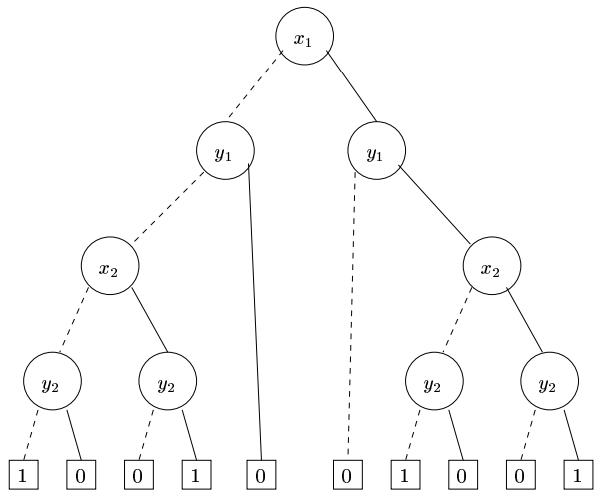
\includegraphics[scale =0.7]{p4.png}
       \caption{Examples of BDD.}
  \end{figure}
%--------------------------------------------------------------------------------------------------------------------------------------

\section{Autarkies}
\label{sec:Autarkies}

\begin{defi}\label{def:autarky}
  Let $F$ be a clause-set. An \textbf{autarky} for $F$ is a partial assignment $\vp$ such that: $\fa C \in F : \var(\vp) \cap \var(C) \neq \es \Ra \vp * \set{C} = \top$ where $\vp * \set{C}$ is given by $\top$ when $\vp$ satisfies $\set{C}$, while otherwise $\vp * \set{C} = \set{D}$, where $D$ is given by taking out all literals from $C$ whose variable is in the domain of $\vp$.
\end{defi}
Namely, whenever a clause is touched by a partial assignment $\vp$, then $\vp$ satisfies it.

\begin{lem}\label{lem:compaut}
  If $\vp, \psi$ are autarkies for $F$, then also the composition $\vp \circ \psi$ is an autarky for $F$.
\end{lem}
\pr If $\vp \circ \psi$ touches a clause $C \in F$ then either:
\begin{enumerate}
\item $\psi$ touches $C$. Now, since $\psi$ is an autarky for $F, C$ is satisfied by $\vp \circ \psi$ since the assignments to variables in var($\psi$) do not  change and still exist in $\vp \circ \psi$.
\item $\psi$ does not touch $C$ and $\vp$ therefore does touch C. Now, since $\vp$ is an autarky for $F$, C is satisfied by $\vp \circ \psi$ since the assignments to variables in $var(\vp) \cap var(C)$ for $\vp$ do not change in $\vp \circ \psi$. 
\end{enumerate}
%--------------------------------------------------------------------------------------------------------------------------------------

\section{The SAT Problem}
\label{sec:The SAT Problem}

\begin{defi}\label{def:sat} Basically, the meaning of \textbf{the SAT problem} is that for a conjunctive normal form $F$, decide whether $F$ is satisfiable or not.
The SAT problem is one of the most versatile NP-complete problems. On the theoretical side, due to its expressiveness and flexibility it 
serves as a tool for many results in complexity theory. On the practical side, NP-completeness of SAT is used “positively”, and many problems 
are translated into  the “universal language” SAT and solved via SAT solvers. 
\end{defi}
%--------------------------------------------------------------------------------------------------------------------------------------
\section{Resolution}
\label{sec:Resolution}

%--------------------------------------------------------------------------------------------------------------------------------------
\section{Unit Resolution}
\label{sec:Unit Resolution}
%--------------------------------------------------------------------------------------------------------------------------------------
\section{Backtracking for SAT}
\label{sec:Backtracking for SAT}
\begin{defi}\label{def:bsat} \textbf{Backtracking} is a general algorithm for finding all (or some) solutions to constraint satisfaction problems, 
that incrementally builds candidates to the solutions, and abandons each partial candidate $c$ ("backtracks") as soon as it determines that c cannot 
possibly be completed to a valid solution. 

In general, a backtracking solver can be described as the following recursive procedure on input $F$:
\begin{enumerate}
\item First we try to simplify $F$ (using for example unit clause elimination as often as we can).
\item Then, using simple criterions, we check whether we immediately see, whether $F$ is satisfiable or
unsatisfiable, in which case we return "satisfiable" resp. "unsatisfiable".
\item Otherwise some "branching variable" v in $F$ is chosen, and it is determined which truth value $\epsilon \in \{ 0, 1\}$ to consider first.
\item Compute $\langle v \to \epsilon \rangle * F$, the result of setting variable v to value $\epsilon$, and apply the procedure recursively to
$\langle v \to \epsilon \rangle * F$. If the result is "satisfiable" then we return "satisfiable".
\item Otherwise, the second branch $\langle v \to \overline{\epsilon} \rangle * F$ has to be considered: If the result is “satisfiable” then
“satisfiable” is returned, otherwise “unsatisfiable”.
\end{enumerate}
\end{defi}

\begin{examp}\label{exp:bdd}
????
\end{examp}
%--------------------------------------------------------------------------------------------------------------------------------------
\section{Methods to Address SAT}
\label{sec:Methods to Address SAT}


%--------------------------------------------------------------------------------------------------------------------------------------
\newpage
\bibliography{my_references}
\bibliographystyle{plainurl}


\end{document}

